\documentclass[12pt,a4paper]{article}
% \usepackage[utf8]{inputenc} % fontspecと併用時は不要
\usepackage[japanese]{babel}
\usepackage{amsmath}
\usepackage{amsfonts}
\usepackage{amssymb}
\usepackage{empheq}
\usepackage{geometry}
\usepackage{graphicx}
\usepackage{enumitem}
\usepackage{fancyhdr}
\usepackage{verbatim}

% 日本語改行設定
\usepackage{xeCJK}
\usepackage{indentfirst}
\setlength{\parindent}{1em}

% 日本語フォント設定
\usepackage{fontspec}
\setmainfont{Hiragino Mincho Pro}
\setsansfont{Hiragino Sans}
\setmonofont{Menlo}
\setCJKmainfont{Hiragino Mincho Pro}
\setCJKsansfont{Hiragino Sans}
\setCJKmonofont{Menlo}
% ページ設定
\geometry{margin=1.5cm}
\setlength{\headheight}{14.70604pt}
\pagestyle{fancy}
\fancyhf{}
\fancyhead[L]{プログラミング応用 期末課題}
\fancyhead[R]{期末課題}
% \fancyfoot[R]{\ifnum\value{page}=1\small（裏面に続く）\fi}
\fancyfoot[C]{\thepage}
\renewcommand{\headrulewidth}{0.4pt}
\renewcommand{\footrulewidth}{0.4pt}

% 問題番号のカウンター
\newcounter{problem}
\setcounter{problem}{0}

% シンプルな問題環境
\newenvironment{problem}[1][]{
    \refstepcounter{problem}
    \vspace{1em}
    \noindent
    \textbf{問\arabic{problem}} #1
    %\vspace{0.5em}
    %\par
}{
    \vspace{1em}
}

\begin{document}

% ヘッダー情報
\begin{center}
    {\Large \textbf{プログラミング応用}}\\[0.5em]
    {\large \textbf{期末課題}}\\[1em]
\end{center}

\noindent\textbf{注意事項}

\begin{itemize}[leftmargin=1em]
    \item 解答はpdf形式でLMSにアップロードしてください (例えば紙に手書きしてスキャンしたものや \TeX をコンパイルしたものなど). ただし, \textbf{手書きの場合は字が汚く読み取れない場合はバツにされる可能性がある}ことに注意してください.
    \item 念のため\textbf{回答用紙には自分の学籍番号と名前を記載しておいてください} (記載していなくても0点にはなりませんが, 確認のため記載してくれると助かります).
    \item 締切：2025年12月\textbf{2日（火）}日本時間13時 (講義の２週間後)
    \item 意図せず\textbf{問題文に不備がある可能性があります}ので, 気軽に問い合わせてください. また, たくさんヒントも出しますので, 積極的に質問してください (SlackのDMも常時受付ます).
    \item 講義中で説明した定理, 補題, 不等式およびこれまでの課題で出題した問題の主張は証明なしに用いてよいですが, 高校や学部1年の範囲では習わないような定理, 補題, 不等式を用いる場合は\textbf{必ずその証明を記載してください} (記載するかしないかが悩ましい場合は必ず相談してください). なお, 全ての問題は講義または課題で登場したもののみで解けます.
    \item 計算量の算出に関しては, $O(\log n)$-bit word RAMモデルを仮定します (詳細は第5回講義資料p.12を参照). 基本的には, アルゴリズムの実行途中に扱う数値が入力長に関して大きくなりすぎなければ大丈夫なので, 普段想定している計算量の算出方法で問題ありません.
    \item アルゴリズムを記述する問題は, 必要があれば乱択アルゴリズムを用いてよいです. その場合は, そのアルゴリズムの成功確率は$\ge 1/2$であるようにしてください\footnote{例えば定数回繰り返して成功確率を増やす場合は「これを$O(1)$回繰り返せば成功確率は$1/2$以上にできる」程度の記載でよい.}.
\end{itemize}

\begin{problem}
グラフ $G=(V,E)$ がグラフ $H=(W,F)$ を含むとは, ある単射 $\phi\colon W\to V$ が存在して, 全ての$H$の辺 $\{a,b\}\in F$ に対して $\{\phi(a),\phi(b)\}\in E$ を満たすことを言う. 隣接行列として与えられた$n$頂点グラフ$G$が次の図\ref{fig:H}で表されるグラフ$H$を含むかどうかを判定する問題を考える.

  \begin{figure}[h]
    \begin{center}
    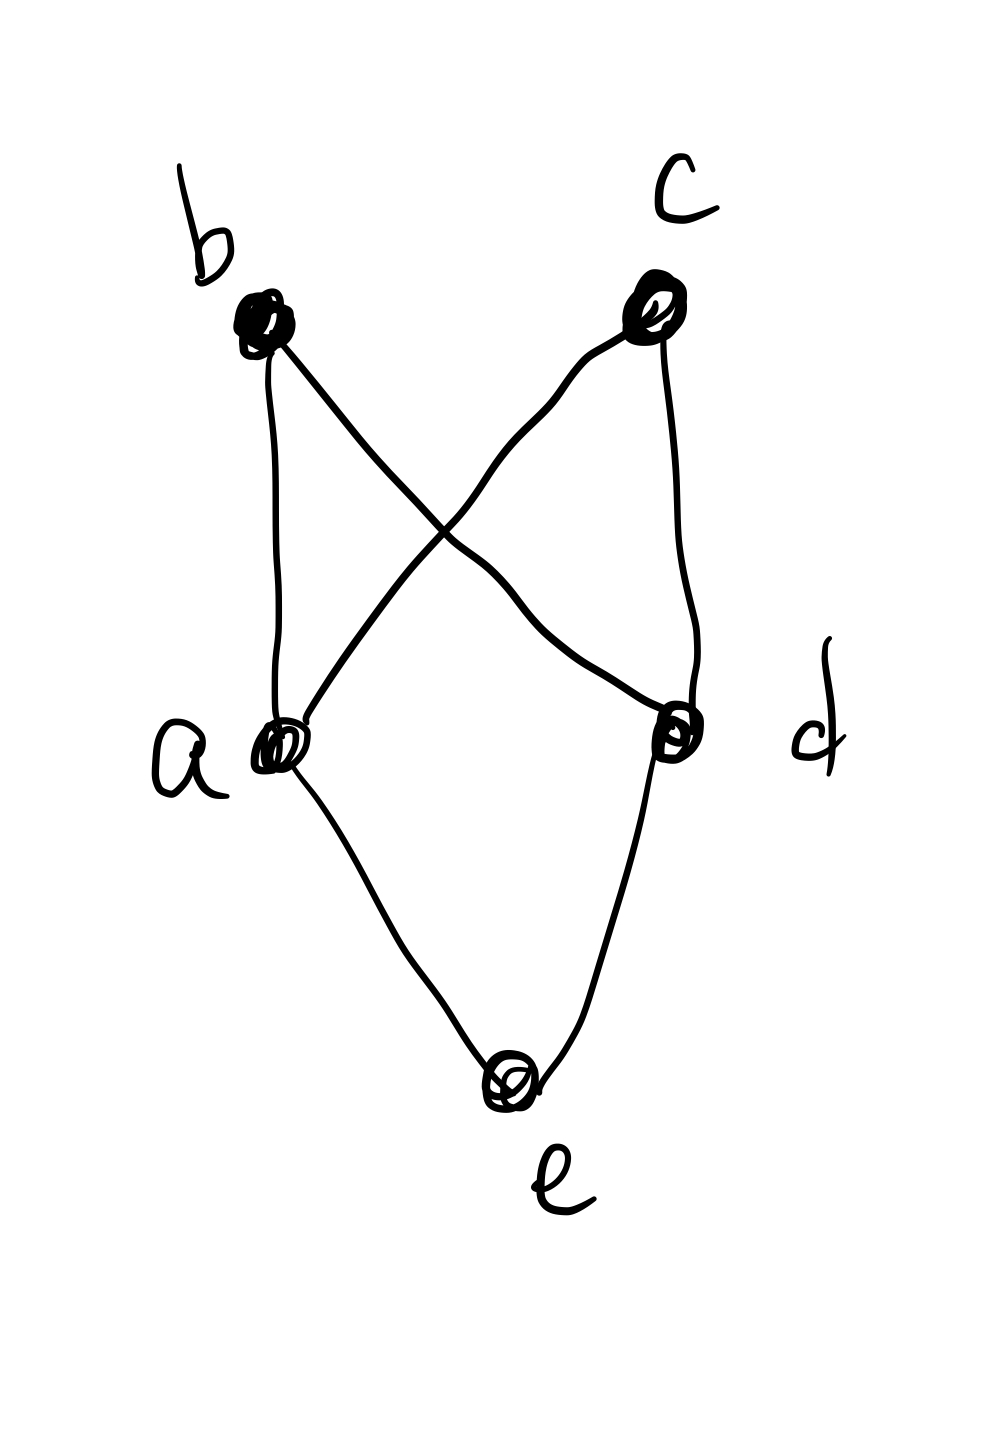
\includegraphics[width=0.14\textwidth]{H.png}
    \caption{グラフ $H$ \label{fig:H}}
    \end{center}
  \end{figure}

  \begin{enumerate}
    \item この問題を $O(n^3)$時間で判定するアルゴリズムを記述せよ.
    \item この問題を $O(n^2)$時間で判定するアルゴリズムを記述せよ.
  \end{enumerate}

\end{problem}

\begin{problem}
$n$個の$n$次元ベクトル $A_1,\dots,A_n \in \mathbb{Z}^{n}$ が与えられる.ただし$n\ge 68$であり, ベクトル$A_i$の各成分の絶対値は高々$n^{100}$である. これらの中から相異なる$68$個のベクトルを選んでその総和を零ベクトルにできるかどうかを $O(n^{34}\log n)$時間で判定するアルゴリズムを記述せよ.
\end{problem}

\begin{problem}
  全点対最短経路問題に対するSeidel法(第4回講義資料参照)において, 2-ホップグラフ$\widetilde{G}$とその二頂点$u,v\in V$を考ぶ. $\widetilde{G}$上の距離$\mathrm{dist}(u,v)$ が偶数のとき, $v$の全ての隣接頂点$i$に対して$\widetilde{\mathrm{dist}}(u,i) \ge \widetilde{\mathrm{dist}}(u,v)$が成り立つことを示せ.
\end{problem}

\begin{problem}
無向グラフ $G=(V,E)$ に含まれる路 $P=(v_0,\dots,v_\ell)$ は, ある $0\le i<j < \ell$ が存在して $(v_i,v_{i+1}) = (v_{j+1},v_j)$ を満たすとき, \textbf{バックトラック}するという (図\ref{fig:backtrack}を参照).
$n$頂点の無向グラフ$G$と二頂点$s,t$が与えられたとき, $G$がバックトラックしない長さがちょうど$247$の$st$路を含むかどうかを, $O(n^3)$時間で判定するアルゴリズムを記述せよ (入力は隣接行列の形で与えられるとする).

  \begin{figure}[h]
    \begin{center}
    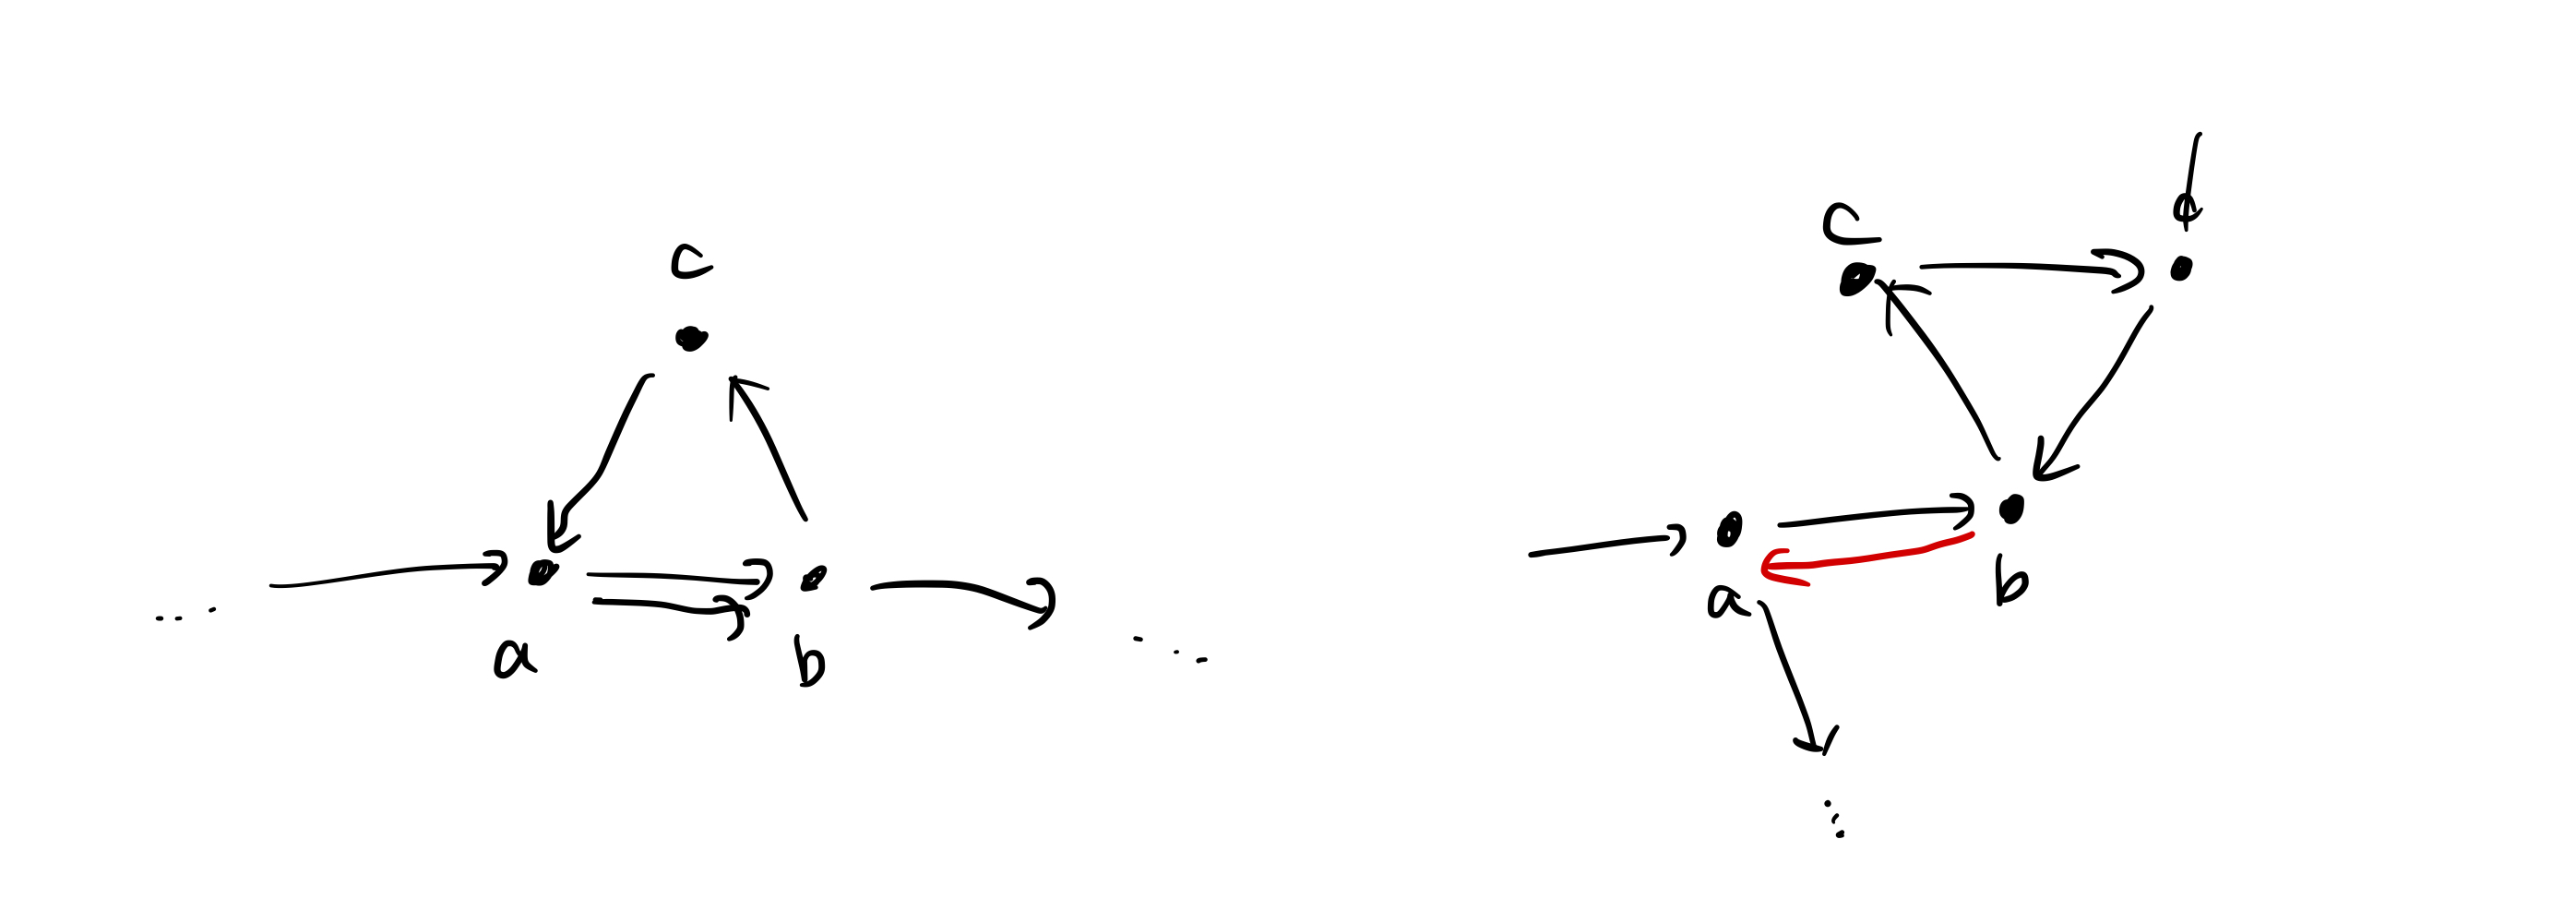
\includegraphics[width=0.66\textwidth]{backtrack.png}
    \caption{右の路は辺$\{a,b\}$を両方の向きで通過しているためバックトラックする.\label{fig:backtrack}}
    \end{center}
  \end{figure}
\end{problem}

\begin{problem}
  第6回課題の問1で考えた主問題(P)とその双対問題(D)を考える:
  \begin{center}
    \begin{minipage}{0.4\textwidth}
      \begin{empheq}[box=\fbox]{align*}
            \text{(P)} \quad \text{minimize} \quad & c^\top x \\
        \text{s.t.} \quad & Ax \ge b \\
                          & x \ge 0
      \end{empheq}
    \end{minipage}
    \quad
    \begin{minipage}{0.4\textwidth}
      \begin{empheq}[box=\fbox]{align*}
              \text{(D)} \quad \text{maximize} \quad & y^\top b \\
          \text{s.t.} \quad & y^\top A \le c^\top \\
                            & y \ge 0
        \end{empheq}
    \end{minipage}
  \end{center}

  第6回課題では非負制約$x\ge 0$を関数$\mathcal{L}^*(y):=\inf_{x\ge 0}\{c^\top x + y^\top (b-Ax)\}$に組み込んで(D)を導出した. 今回は非負制約を行列を用いて書き換えた問題(P')について, 第6回講義資料と同様の方法で双対問題を導出せよ:
    \begin{empheq}[box=\fbox]{align*}
        \text{(P')} \quad \text{minimize} \quad & c^\top x \\
    \text{s.t.} \quad & \begin{bmatrix} A \\
    I \end{bmatrix} x \ge \begin{bmatrix} b \\
    0 \end{bmatrix}
  \end{empheq}
  ただし, $I\in\mathbb{R}^{n\times n}$は単位行列である. また, $Ax\ge b$に対応する双対変数を$y\in\mathbb{R}^m$, $Ix\ge 0$に対応する双対変数を$z\in\mathbb{R}^n$とせよ.
  さらに, この導出した双対問題を(D')としたとき, (D)と(D')が等価であることを示せ. つまり, 一方の最適解を用いて他方の最適解を構成できることを示せ.

\end{problem}

\end{document}